\documentclass[tikz,border=10pt]{standalone}
\usepackage{amsmath}
\usetikzlibrary{arrows.meta,positioning,backgrounds,patterns}
\begin{document}
% Shared chapter style: white canvas, sans-serif text, 0.9 pt strokes,
% restrained rounded process boxes, and 3 mm Latex arrowheads.
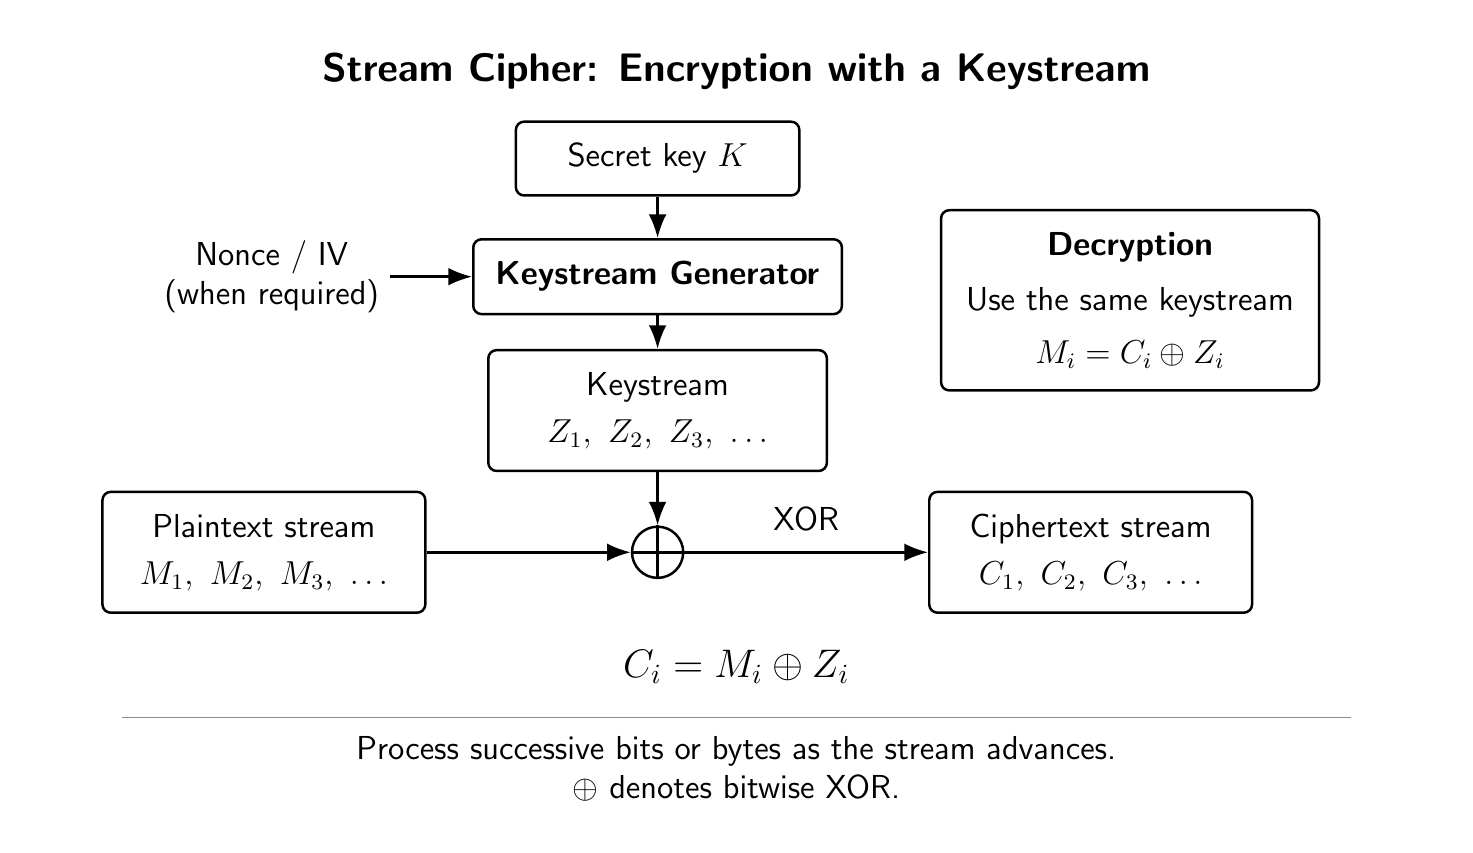
\begin{tikzpicture}[
    font=\sffamily\large, line width=0.9pt,
    background rectangle/.style={fill=white,draw=none},
    show background rectangle,
    box/.style={draw,fill=white,rounded corners=3pt,align=center,inner sep=8pt},
    data/.style={draw,fill=white,align=center,minimum width=2.4cm,minimum height=0.85cm},
    enc/.style={box,minimum width=2.4cm,minimum height=1.05cm},
    arrow/.style={-{Latex[length=3mm]},line width=0.9pt},
    title/.style={font=\sffamily\Large\bfseries,align=center},
    note/.style={align=center},
    repeated/.style={fill=black!14,line width=1.3pt}
]
\path[use as bounding box] (-9,-5.0625) rectangle (9,5.0625);

\node[title] at (0,4.5) {Stream Cipher: Encryption with a Keystream};
\node[box,minimum width=3.6cm] (key) at (-1,3.4) {Secret key $K$};
\node[box,minimum width=4.3cm,minimum height=0.95cm] (gen) at (-1,1.9)
    {\textbf{Keystream Generator}};
\draw[arrow] (key.south) -- (gen.north);
% Practical generators commonly also take a public nonce / IV.
\node[note] (nonce) at (-5.9,1.9) {Nonce / IV\\(when required)};
\draw[arrow] (nonce.east) -- (gen.west);
\node[box,minimum width=4.3cm] (z) at (-1,0.2)
    {Keystream\\[3pt]$Z_1,\ Z_2,\ Z_3,\ \ldots$};
\draw[arrow] (gen.south) -- (z.north);
% A circle with crossing strokes is the conventional XOR junction.
\node[draw,circle,fill=white,minimum size=0.65cm,inner sep=0pt] (xor) at (-1,-1.6) {};
\draw (xor.north) -- (xor.south);
\draw (xor.west) -- (xor.east);
\draw[arrow] (z.south) -- (xor.north);
\node[box,minimum width=4.1cm] (m) at (-6,-1.6)
    {Plaintext stream\\[3pt]$M_1,\ M_2,\ M_3,\ \ldots$};
\node[box,minimum width=4.1cm] (c) at (4.5,-1.6)
    {Ciphertext stream\\[3pt]$C_1,\ C_2,\ C_3,\ \ldots$};
\draw[arrow] (m.east) -- (xor.west);
\draw[arrow] (xor.east) -- node[above=4pt] {XOR} (c.west);
\node[box,minimum width=4.8cm,align=center] at (5,1.6)
    {\textbf{Decryption}\\[6pt]Use the same keystream\\[5pt]
     $M_i=C_i\oplus Z_i$};
\node[font=\sffamily\Large] at (0,-3.05) {$C_i=M_i\oplus Z_i$};
\draw[black!45,line width=0.6pt] (-7.8,-3.7) -- (7.8,-3.7);
\node[note] at (0,-4.35)
    {Process successive bits or bytes as the stream advances.\\
     $\oplus$ denotes bitwise XOR.};
\end{tikzpicture}
\end{document}
